% This is a LaTeX thesis template for Monash University.
% to be used with Rmarkdown
% This template was produced by Rob Hyndman
% Version: 6 September 2016

\documentclass{monashthesis}

%%%%%%%%%%%%%%%%%%%%%%%%%%%%%%%%%%%%%%%%%%%%%%%%%%%%%%%%%%%%%%%
% Add any LaTeX packages and other preamble here if required
%%%%%%%%%%%%%%%%%%%%%%%%%%%%%%%%%%%%%%%%%%%%%%%%%%%%%%%%%%%%%%%

\author{Priyanga Dilini Talagala}
\title{Anomaly Detection in Streaming Time Series Data}
\degrees{B.Sc. (Hons), University of Sri Jayewardenepura, Sri Lanka}
\def\degreetitle{Doctor of Philosophy}
% Add subject and keywords below
\hypersetup{
     %pdfsubject={The Subject},
     %pdfkeywords={Some Keywords},
     pdfauthor={Priyanga Dilini Talagala},
     pdftitle={Anomaly Detection in Streaming Time Series Data},
     pdfproducer={Bookdown with LaTeX}
}


\bibliography{thesisrefs}

\usepackage{amsthm}
\newtheorem{theorem}{Theorem}[chapter]
\newtheorem{lemma}{Lemma}[chapter]
\newtheorem{corollary}{Corollary}[chapter]
\newtheorem{proposition}{Proposition}[chapter]
\newtheorem{conjecture}{Conjecture}[chapter]
\theoremstyle{definition}
\newtheorem{definition}{Definition}[chapter]
\theoremstyle{definition}
\newtheorem{example}{Example}[chapter]
\theoremstyle{definition}
\newtheorem{exercise}{Exercise}[chapter]
\theoremstyle{remark}
\newtheorem*{remark}{Remark}
\newtheorem*{solution}{Solution}
\let\BeginKnitrBlock\begin \let\EndKnitrBlock\end
\begin{document}

\pagenumbering{roman}

\titlepage

{\setstretch{1.2}\sf\tighttoc\doublespacing}

\hypertarget{copyright-notice}{%
\chapter*{Copyright Notice}\label{copyright-notice}}
\addcontentsline{toc}{chapter}{Copyright Notice}

© Priyanga Dilini Talagala (2019).

I certify that I have made all reasonable efforts to secure copyright permissions for third-party content included in this thesis and have not knowingly added copyright content to my work without the owner's permission.

Except as provided in the Copyright Act 1968, this thesis may not be reproduced in any form without the written permission of the author.

\hypertarget{abstract}{%
\chapter*{Abstract}\label{abstract}}
\addcontentsline{toc}{chapter}{Abstract}

Anomaly detection has wide variations in problem formulations, which demand different analytical approaches. Despite the ever-increasing attention and resources devoted to the area of anomaly detection, some challenges are not supported by the existing frameworks and algorithms. This thesis reduces this gap by introducing three new algorithms for anomaly detection with special reference to their capabilities, competitive features and target applications.

This thesis offers four fundamental contributions. First, it proposes an improved algorithm for anomaly detection in high-dimensional data. It outperforms the state-of-the-art methods in many examples in terms of both accuracy and computational efficiency, while retaining a valid probabilistic interpretation for the anomalous threshold. Further, many existing algorithms have been specifically developed for the batch scenario, where it is assumed that all available data have been collected prior to analysis. However, with the recent rapid advances in data collection technology, streaming data are now becoming increasingly important and pose various challenges due to nonstationarity, noisy signals, large volume, high velocity, incomplete events and online support. To meet these challenges, as a second contribution, the thesis proposes another algorithm that provides early detection of anomalies within a large collection of streaming time series data. This algorithm includes a novel approach that adapts to nonstationarity. Third, it proposes a new algorithm to detect anomalies, caused by technical issues, in water-quality data from in situ sensors. Fourth, with the aim of facilitating reproducible research, the first, second and third algorithms are implemented in three open source R packages: \texttt{stray}, \texttt{oddstream} and \texttt{oddwater}, respectively. Using various synthetic and real datasets, this thesis demonstrates the wide applicability and usefulness of the three algorithms.

In \texttt{stray}, an anomaly is defined as an observation that deviates markedly from the majority with a large distance gap. This improved unsupervised algorithm for high-dimensional data is based on distance measures and the extreme value theory. In \texttt{oddstream}, an anomaly is defined as an observation that is very unlikely, given the recent distribution of a given system. In this algorithm, a boundary for the system's typical behaviour is calculated using the extreme value theory. Then, a sliding window is used to test newly arrived data. The model uses time series features as inputs and a density-based comparison to locate nonstationarity. \texttt{Oddwater} involves an application where anomaly detection is performed using turbidity, conductivity and river level data collected from rivers flowing into the Great Barrier Reef lagoon, Australia.

The algorithm, \texttt{stray}, which is specially designed for high-dimensional data, addresses the limitations of the state-of-art-method, the \texttt{HDoutliers} algorithm. Using various applications, this thesis demonstrates how \texttt{stray} can be used to detect anomalies in other data types, such as temporal data and streaming data. Applications of \texttt{oddstream} with data obtained using fibre optic cables showed that the framework has the ability to provide early detection of anomalies in large streaming nonstationary data. \texttt{Oddwater} successfully identified abrupt changes caused by technical outliers in water-quality sensors, while maintaining very low false detection rates.

\hypertarget{publications-during-enrolment}{%
\chapter*{Publications During Enrolment}\label{publications-during-enrolment}}
\addcontentsline{toc}{chapter}{Publications During Enrolment}

This thesis by publication is built around four articles which are at different stages of publication.

\begin{enumerate}
\def\labelenumi{\arabic{enumi}.}
\item
  Chapter \ref{ch:stray} has been submitted to \emph{Computational Statistics \& Data Analysis} for possible publication.

  Talagala, P. D., Hyndman, R. J. \& Smith-Miles, K. (2019). Anomaly Detection for High Dimensional Data. \emph{arXiv preprint arXiv:1908.04000.}
\item
  Chapter \ref{ch:oddstream} has been accepted for publication in the \emph{Journal of Computational and Graphical Statistics} and is currently in press.

  Talagala, P. D., Hyndman, R.J., Smith-Miles, K., Kandanaarachchi, K., \& Muñoz, M.A., (2019) Anomaly Detection in Streaming Nonstationary Temporal Data, \emph{Journal of Computational and Graphical Statistics}, DOI: 10.1080/10618600.2019.1617160.

  I won the ACEMS Business Analytics prize 2018 for this work.
\item
  Chapter \ref{ch:oddwater_features} has been revised and resubmitted to the \emph{Water Resources Research} for possible publication.

  Talagala, P. D., Hyndman, R. J., Leigh, C., Mengersen, K., \& Smith-Miles, K. (2019). A feature-based framework for detecting technical outliers in water-quality data from in situ sensors. \emph{arXiv preprint arXiv:1902.06351.}
\item
  Chapter \ref{ch:oddwater_main} is published in the \emph{Science of the Total Environment}.

  Leigh, C., Alsibai, O., Hyndman, R. J., Kandanaarachchi, S., King, O. C., McGree, J. M., Neelamraju, C., Strauss, J., Talagala, P.D., Turner, R.D., Mengersen, K., \& Peterson, E.E. (2019). A framework forautomated anomaly detection in high frequency water-quality data from in situ sensors. \emph{Science of the Total Environment} 664, 885-898.
\end{enumerate}

The contribution in Chapters \ref{ch:stray}, \ref{ch:oddstream} and \ref{ch:oddwater_features} of this thesis were presented at the following events:

\begin{itemize}
\tightlist
\item
  37th International Symposium on Forecasting 2017, Cairns, Australia.
\item
  Young Statisticians Conference 2017, Tweed Heads NSW, Australia. \newline A Statistical Society of Australia travel award grant was received to attend the conference.
\item
  Young Stats Showcase hosted by the Statistical Society of Australia, Victorian Branch, Australia, in September 2017.
\item
  38th International Symposium on Forecasting 2018, Boulder, Colorado, USA. \newline
  An International Institute of Forecasters travel award grant was received to attend the conference.
\item
  2018 Joint Statistical Meetings (JSM2018), Vancouver, British Columbia, Canada
\item
  useR! 2018, Brisbane, Australia.
\item
  Joint International Society for Clinical Biostatistics and Australian Statistical Conference 2018 (ISCB ASC18), Melbourne, Australia. \newline I won the EJP Pitman Young Statisticians Prize 2018, Merit Award `for the outstanding talk presented by a \emph{Young Statistician} at an Australian Statistical Conference'.
\item
  39th International Symposium on Forecasting, Thessaloniki, Greece. \newline An International Institute of Forecasters travel award grant was received to attend the conference.
\item
  useR! 2019, Toulouse, France.
  \newline A conference diversity scholarship was received to attend the conference.
\end{itemize}

\hypertarget{declaration}{%
\chapter*{Declaration}\label{declaration}}
\addcontentsline{toc}{chapter}{Declaration}

I hereby declare that this thesis contains no material which has been accepted for the award of any other degree or diploma at any university or equivalent institution and that, to the best of my knowledge and belief, this thesis contains no material previously published or written by another person, except where due reference is made in the text of the thesis.

This thesis includes 2 original papers published in peer reviewed journals and 2 submitted publications. The core theme of the thesis is anomaly detection in streaming time series data. The ideas, development and writing up of all the papers (with the exception of Chapter 5) in the thesis were the principal responsibility of myself, the student, working within the Department of Econometrics and Business Statistics, Monash University, under the supervision of Professor Rob J. Hyndman and Professor Kate Smith-Miles.

The inclusion of co-authors reflects the fact that the work came from active collaboration between researchers and acknowledges input into team-based research.

In the case of Chapter 2-5 my contribution to the work involved the following:

\begin{table}[H]
\small
\begin{tabular}{|p{0.5cm}|p{2cm}|p{1.5cm}|p{4cm}|p{3.5cm}|p{1cm}|}
\rowcolor[HTML]{000000} 
{\color[HTML]{FFFFFF} \textbf{Thesis Chapter} } & {\color[HTML]{FFFFFF} \textbf{Publication Title} } & {\color[HTML]{FFFFFF} \textbf{Status (published, in press, accepted or returned for revision)} } & {\color[HTML]{FFFFFF} \textbf{Nature and \% of student contribution}}& {\color[HTML]{FFFFFF} \textbf{Co-author name(s) Nature and \% of Co-author’s contribution}} & {\color[HTML]{FFFFFF} \textbf{Co-author(s), Monash student Y/N }} \\ \hline
 2 & Anomaly Detection for High Dimensional Data   &  Submitted  &  Formulating the approach, construction of research design, implementation, data analysis and interpretation, software development, writing the first draft (80\%)    & 1) Rob J. Hyndman, input into manuscript (10\%) \newline 2) Kate Smith-Miles, input into manuscript (10\%)  & N
 \\ \hline
3  & Anomaly Detection in Streaming Non-stationary Temporal Data  & Published   & Formulating the approach, construction of research design, implementation, data analysis and interpretation, software development, writing the first draft (80\%)   & 1) Rob J. Hyndman, input into manuscript (10\%) \newline 2) Kate Smith-Miles, input into manuscript (5\%) \newline 3) Sevvandi Kandanaarachchi and Mario A. Mu\~noz, input into manuscript (5\%)  & N  
\\ \hline
4  & A feature-based procedure for detecting technical outliers in water-quality data from in situ sensors  &  Revised and resubmitted & Formulating the approach, construction of research design, implementation, data analysis and interpretation, software development, writing the first draft (80\%)  & 1) Rob J. Hyndman, input into manuscript (10\%) \newline  2) Catherine Leigh, Kerrie Mengersen and Kate Smith-Miles, input into manuscript (10\%) & N  
\\ \hline
5  & A framework for automated anomaly detection in high frequency water-quality data from in situ sensors  &    Published &  Formulating the feature based anomaly detection approach: implementation, data analysis and interpretation, software development, writing the first draft of the feature based approach related parts. Developing a Shiny web application to explore data. Data preprocessing. (30\%)    & (1) Catherine Leigh, input into manuscript (40\%) \newline  2) Rob J. Hyndman, input into manuscript (10\%) \newline
3) Other co-authors, input into manuscript (20\%) & N  
\\ \hline
\end{tabular}
\end{table}

I have not renumbered sections of submitted or published papers in order to generate a consistent presentation within the thesis.

\textbf{Student name:} Priyanga Dilini Talagala \hspace{3cm}\textbf{Date:}19.08.2019

\hypertarget{acknowledgements}{%
\chapter*{Acknowledgements}\label{acknowledgements}}
\addcontentsline{toc}{chapter}{Acknowledgements}

Over the past few years, with my experience on anomaly detection, I realised how important the support from the surrounding points is for a point to stand out as an anomaly, just like my support system around me supported me to make this thesis a reality. Now, it is my great pleasure to thank everyone who made this thesis possible.

I am deeply grateful to my supervisor Professor Rob J. Hyndman. Your valuable guidance and your way of thinking about, and doing, research continue to inspire me and shaped my thinking about all facets of this research. My research style, my research focus, my research toolkit -- they all have their own roots in your mentorship. I am also very grateful to my co-supervisor Professor Kate Smith-Miles from University of Melbourne, Australia, who always raised important questions I never would have considered. I am truly blessed to have you two throughout this very special journey. Your influence on my thinking about research from different angles and boosting my confidence is beyond estimation.

Chapters 3 and 4 are based on the collaborative research project carried out with the Queensland University of Technology and the Queensland Department of Environment and Science, Great Barrier Reef Catchment Loads Monitoring Program. I consider myself very lucky to have had such a great opportunity to work on this project with many wonderful mentors, including Professor Kerrie Mengersen, Dr Erin Peterson and Dr.~Catherine Leigh. Thank you for your thoughtful critiques, support, guidance, encouragement and generous hospitality during my visit to Queensland University of Technology, Australia, in April 2018. It was pure joy working with you all.

I was able to learn so much at, Monash University because of financial support from the Monash Graduate Scholarship and the Faculty Graduate Research scholarship. This assistance has provided me many unique opportunities that I will always be thankful for. I am also thankful to ARC Centre of Excellence for Mathematical and Statistical Frontiers (ACEMS) for funding my visit to Queensland to work on the water-quality project and the Australian Research Council through the Linkage Project LP160101885 for funding the research study in Chapter 1 of this thesis. I am also thankful to the Queensland Department of Environment and Science; in particular, the Great Barrier Reef Catchment Loads Monitoring Program for the data, and the staff from Water Quality and Investigations for their input on Chapters 3 and 4 of this thesis. Further, this research was supported in part by the Monash eResearch Centre and eSolutions Research Support Services through the use of the MonARCH (Monash Advanced Research Computing Hybrid) HPC Cluster. I want to thank them for their valuable contribution.

I am also very thankful to my thesis committee, Professor Gael Martin, Professor Farshid Vahid, Professor George Athanasopoulos and Professor Xueyan Zhao, for their valuable feedback and suggestions. I am also grateful to David Hill and the many anonymous reviewers who read the manuscripts presented in Chapters 3, 4 and 5 and generously provided insights and suggestions to improve our work. I am also thankful to all my co-authors for their valuable contribution and collaborations. Special thanks to Cathy Morgan and Elite Editing for helping in copy editing and clarifying the manuscripts. The editorial intervention by Elite Editing was restricted to Standards D and E of the Australian Standards for Editing Practice.

I take this opportunity to thank the Statistical Society of Australia (SSA) for the travel grant to present at the Young Statisticians Conference 2017, Tweed Heads, NSW, Australia; the International Institute of Forecasters for the travel grant to present at the 38th International Symposium on Forecasting, Boulder, Colorado, USA and the travel grant to present at the 39th International Symposium on Forecasting, Thessaloniki, Greece; useR! 2019 for the travel grant to present at useR! 2019, Toulouse, France; and Monash EBS travel grant to present at JSM 2018, Vancouver, Canada. Each of these conferences is a unique experience and allowed me to share my research findings with a wider community. These conferences helped me significantly to attract the attention of peers and experts in my field, and the questions, comments and suggestions I received from both academic and industry-oriented researchers helped me considerably in improving my work.

During my stay at Monash, the department administrative staff members, especially Clare Livesey, were very supportive and positive regarding every request. The Monash graduate research team was also very helpful and timely with all requests and I want to thank them for their assistance.

Special thanks to my sister, Thiyanga Talagala, who was there with, and for me, every step of the way, sharing many hats as siblings, schoolmates, college mates, workmates and office mates. I was extremely lucky to have an opportunity to have her by my side and share our latest and most precious hats as academic sisters and batch mates together at Monash University.
Deeply grateful to our parents whom I love, admire, respect and find comfort in beyond words; you are a pillar of strength for me. All three of you have had a bigger influence on this thesis than you might realise.

\clearpage\pagenumbering{arabic}\setcounter{page}{0}

\hypertarget{ch:intro}{%
\chapter{Introduction}\label{ch:intro}}

Anomaly detection is an important research topic that has been explored within diverse research areas and application domains. The presence of anomalies in data can lead to biased parameter estimation, model misspecification and misleading results if classical analysis techniques are blindly applied \autocite{abuzaid2013detection,ben2005outlier}. Conversely, anomalies themselves can be the main carriers of significant and often critical information and the identification of these critical points can be the main purpose of many investigations in fields such as fraud detection (e.g., credit card frauds and network intrusion), object tracking (e.g., flight tracking), system health monitoring (e.g., machine breakdown and power cable leakages) and environmental monitoring (e.g., water quality, bushfire, earthquake and volcanic eruption) \autocite{gupta2014outliersurvey}. Further, owing to rapid advances in data collection technology it has become increasingly common for organisations to be dealing with data that stream in large quantities. Therefore, the overall focus of this thesis is on detecting anomalies in streaming time series data.

\hypertarget{background}{%
\section{Background}\label{background}}

This section reviews the background work on anomaly detection for
streaming time series data and lays the foundation for the work presented in Chapters \ref{ch:stray}--\ref{ch:oddwater_main}

\hypertarget{definitions-found-in-the-literature}{%
\subsection{Definitions Found in the Literature}\label{definitions-found-in-the-literature}}

Solutions to the problem of detecting unusual behaviours in systems of interest can be influenced heavily by the way in which anomalies are defined. Three terms are used commonly and interchangeably in the literature to describe work related to the topic: \emph{novelty} \autocite{clifton2011novelty,hugueny2013novelty}, \emph{anomaly} \autocite{hyndman2015large,kumar2016adaptive} and \emph{outlier} \autocite{schwarz2008wind,wilkinsonvisualizing}. However, \textcite{faria2016novelty} differentiate between these three terms, using the terms anomaly and outlier to refer to the idea of an undesired pattern but novelty to refer to the emergence of a new concept that needs to be incorporated into the typical behaviour of the system. In line with this view, \textcite{chandola2009anomaly} define an anomaly as a pattern in the data that does not conform to the expected behaviour but a novelty as an unobserved pattern that is typically incorporated into the model of the typical behaviour of a given system when it is detected. However, \textcite{gama2010knowledge} points out that a substantial number of examples is required as evidence of the appearance of a novelty before it should be incorporated into the model of the typical behaviour of a given system. Thus, the sparse examples that differ considerably from the `typical' behaviour can all be considered anomalies or outliers, since there is no guarantee that they represent a new
`typical' behaviour of the system \autocite{faria2016novelty}. \textcite{lavin2015evaluating} define anomalies in streaming data, with respect to their past behaviour, as
patterns that do not conform to the past behaviours of the system. As a result, a new behaviour may be anomalous at first, but it ceases to be
anomalous if the new `typical' pattern continues to exist, and ultimately
ends up being a novelty rather than an anomaly or an outlier.

\textcite{grubbs1969procedures} defines an anomaly as an observation that deviates markedly from other members of the sample. However, this deviation can be defined in terms of either distance or density. \textcite{burridge2006additive}, \textcite{wilkinsonvisualizing} and \textcite{schwarz2008wind} have all proposed methods for
anomaly detection by defining an anomaly in terms of distance. In contrast, \textcite{hyndman1996computing}, \textcite{clifton2011novelty} and \textcite{hugueny2013novelty} have proposed methods that define an anomaly with respect to either the density or the chance of the occurrence of observations.

\hypertarget{representation-of-time-series}{%
\subsection{Representation of Time Series}\label{representation-of-time-series}}

According to \textcite{fulcher2014highly}, the representation of time series is twofold: instance-based and feature-based.

The instance-based representation of time series is the most
straightforward and has been used by many researchers in the data mining community. Under this representation, if two time series are to be compared, a distance metric between the two time series is defined that leads to a direct comparison of the ordered values of the two time series. The methods proposed by \textcite{wilkinsonvisualizing}, \textcite{clifton2011novelty} and \textcite{hugueny2013novelty} are all based on this representation of time series.

In contrast to the instance-based representation of time series, the feature-based representation of time series involves representing a given time series in terms of its properties, measured using different statistical operations, thereby transforming a temporal problem into a static problem \autocite{fulcher2013highly}. After extracting features, further analysis is based on these extracted features. Thus, this representation can allow an algorithm to compare time series of different lengths and/or starting points, because it can transform time series of any length or starting point into a vector of features of a fixed size. Recently, researchers such as \textcite{wang2006characteristic}, \textcite{fulcher2012highly} and \textcite{hyndman2015large} have paid a considerable amount of attention to the feature-based representation of time series, since it helps to reduce the dimension of the original multivariate time series problem via features that encapsulate the dynamic properties of the individual time series efficiently.

\hypertarget{extreme-value-theory}{%
\subsection{Extreme Value Theory}\label{extreme-value-theory}}

The algorithms proposed in Chapters \ref{ch:stray}, \ref{ch:oddstream} and \ref{ch:oddwater_features} are based on th extreme value theory, a branch of probability theory that relates to the behaviour of extreme order statistics in a given sample \autocite{galambos2013extreme}. In contrast to traditional data analysis, where the primary focus is on the observations in the central region of the distribution, extreme value theory focuses primarily on modelling the distribution of extreme order statistics in a given sample \autocite{pinto2016advanced,clifton2009novelty}. The central limit theorem is one of the most striking limit theorems in statistics. Its ability to approximate the distribution of the sample mean irrespective of the parent distribution of the original random variable is the property that makes this theorem so remarkable \autocite{coles2001introduction}. Analogous arguments are used in the extreme value theory to approximate distributions of extreme order statistics in a given sample.

\hypertarget{key-results-of-classical-extreme-value-theory}{%
\subsection{Key Results of Classical Extreme Value Theory}\label{key-results-of-classical-extreme-value-theory}}

Consider a set of \(m\) independent and identically distributed (iid) data, \(\;\textbf{X}= \{x_{1}, x_{2}, \dots,\) \(x_{m}\},\) which has its own cumulative distribution function (CDF), \(F\), and an associated probability density function (pdf), \(f\). In classical extreme value theory, \(x_{i} \in \Re\) (univariate). Let \(X_{max}= max(\textbf{X})\) and \(X_{min}= min(\textbf{X})\). The extreme value theory focuses on the statistical behaviour of these quantities. Hereafter, the discussion will focus on \(X_{max}\) (\(X_{min}\) will be referred to only when necessary), because it simplifies the discussion, but a similar argument can be applied to \(X_{min}\) as well.

The distribution of \(X_{max}\) can be investigated by taking several random samples of size \(m\) from a given distribution, recording the maximum of each sample and constructing a density plot of the maxima. Figure \ref{fig:EVDchange} (reproduced from \textcite{hugueny2013novelty}, p.~87) shows the empirical distributions of minima and maxima for the standard Gaussian distribution (left), and of maxima for the standard exponential distribution (right) for series of sizes \(m\). Each density plot is based on \(10^6\) data points. Consider the case of \(m=1\), where we observe only one data point from \(f\) in each trial. The corresponding density plot approximates the generative distribution \(f\), because the maximum of a singleton set \(\{x\}\) is simply \(x\). However, the density plots for maxima move to the right as \(m\) increases, implying that the expected location of the sample maximum on the x-axis increases as more data are observed from \(f\). Let \(H^{+}\) denote the distribution function of \(X_{max}\). This is termed the \emph{extreme value distribution} (EVD), because it describes the expected location of the maximum of a sample of size \(m\) generated from \(f\) \autocite{clifton2011novelty}. The Fisher--Tippett Theorem \autocite{fisher1928limiting}, which is the basis of classical extreme value theory, explains the possibilities for this \(H^{+}\).

\begin{figure}[h]

{\centering 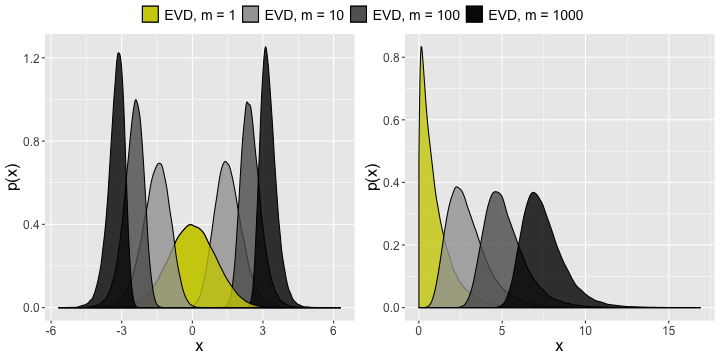
\includegraphics[width=1\linewidth]{figure/EVDchange-1} 

}

\caption{Empirical distributions of $10^6$ minima and maxima for the standard Gaussian distribution (left), and of maxima for the standard exponential distribution (right). (Reproduced from Hugueny, 2013, p.87.)}\label{fig:EVDchange}
\end{figure}

\BeginKnitrBlock{theorem}[Fisher-Tippett theorem, limit laws for maxima]
\protect\hypertarget{thm:fisherTippet}{}{\label{thm:fisherTippet} \iffalse (Fisher-Tippett theorem, limit laws for maxima) \fi{} }(Theorem 3.2.3 in \emph{\textcite{embrechts2013modelling}}, p.~121; the notations have been changed for consistency within this thesis.)

Let \(\textbf{X}= \{x_{1}, x_{2},\dots ,x_{m}\}\) be a sequence of iid random variables and \(X_{max}= max(\textbf{X})\). If there exists a centring constant \(d_{m} (\in\Re)\) and normalising constant \(c_{m} (>0)\), and some non-degenerate distribution function \(H^{+}\) (`+' refers to the distribution of maxima) such that:
\begin{equation*}
c_{m}^{-1}(X_{max}-d_{m}) \xrightarrow{\text{d}} H^{+},
\end{equation*}

then \(H^{+}\) belongs to one of the following three distribution function types:

\(\;\;\;\;\;\;\;\;\;\;\;\;\;\;\;\;\;\;\;\;\text{\textit{Fr\'{e}chet}}:\;\;\;\;\varPhi_{\alpha}^{+}(x)\;\;\;=\; \begin{cases} 0, \;\;\;\;\;\;\;\;& x \leqslant 0\\ exp\{-x^{-\alpha}\}, \;\;\;\; & x>0 \end{cases}\;\;\;\;\;\;\alpha>0\)

\(\;\;\;\;\;\;\;\;\;\;\;\;\;\;\;\;\;\;\;\;\text{\textit{Weibull}}:\;\;\;\;\varPsi_{\alpha}^{+}(x)\;=\; \begin{cases} exp\{-(-x)^{\alpha}\},& x \leqslant 0\\ 1, & x>0 \end{cases}\;\;\;\;\;\;\alpha>0\)

\(\;\;\;\;\;\;\;\;\;\;\;\;\;\;\;\;\;\;\;\;\text{\textit{Gumbel}}:\;\;\;\varLambda^{+}(x)\;\;\;\;=\;\; exp\{-e^{-x}\},\;\;\;\;\;\;\;\;\;x \in\Re.\\\)
\EndKnitrBlock{theorem}

\BeginKnitrBlock{definition}[Extreme value distribution and extremal random variable]
\protect\hypertarget{def:evdrv}{}{\label{def:evdrv} \iffalse (Extreme value distribution and extremal random variable) \fi{} }(Definition 3.2.6 in \textcite{embrechts2013modelling}, p.~124)

The distribution functions \(\varPhi_{\alpha}, \varPsi{\alpha}\) and \(\varLambda\) as presented in Theorem \ref{thm:fisherTippet} are called standard extreme value distributions and the corresponding random variables, standard extremal random variables. Distribution functions of the types of \(\varPhi_{\alpha}, \varPsi{\alpha}\) and \(\varLambda\) are extreme value distributions; the corresponding random variables are extremal random variables.

\begin{flushright}
    $\square$
   \end{flushright}
\EndKnitrBlock{definition}

From Theorem \ref{thm:fisherTippet}, it can be observed that the extreme value distributions are implicitly parameterised by \(m\), the size of the sample from which the extrema is taken. Therefore, different values of \(m\) will yield different extreme value distributions \autocite{clifton2011novelty}.

\BeginKnitrBlock{definition}[Maximum domain of attraction]
\protect\hypertarget{def:MDA}{}{\label{def:MDA} \iffalse (Maximum domain of attraction) \fi{} }(Definition 3.3.1 in \textcite{embrechts2013modelling}, p.~128; the notations have been changed for consistency within this thesis.)

We say that the rv \(X\) (the distribution function \(F\) of \(X\) or the distribution of \(X\)) belongs to the maximum domain of attraction of the extreme value distribution \(H^{+}\) if there exist constants \(c_{n} > 0\), \(d_{n} \in \Re\) such that:

\begin{center}
    $c_{m}^{-1}(X_{max}-d_{m}) \underrightarrow{d} H^{+}$.
\end{center}

We write \(X \in MDA(H^{+}) \;\;(F \in MDA(H^{+}))\).

\begin{flushright}
    $\square$
\end{flushright}
\EndKnitrBlock{definition}

The following properties, highlighted by \textcite{embrechts2013modelling}, will assist in deciding the maximum domain of attraction of the three extreme value distributions to which \(X\) belongs. Let \(x_{F} = \text{sup}{\{x \in \Re : F(x) < 1\}}\) denote the right endpoint of \(F\).

\begin{itemize}
\item
  All distribution functions \(F \in MDA(\varPhi_{\alpha}^{+})\) have an infinite right endpoint \(x_{F} = \infty\) (the tail decreases like a power low). The Pareto, F, Cauchy and log-gamma distribution functions are just a few examples covered by the maximum domain of attraction of the \(\text{Fr\'{e}chet}\) distribution.
\item
  All distribution functions \(F \in MDA(\varPsi_{\alpha}^{+})\) have a finite right endpoint \(x_{F} < \infty\) (truncated tail). The uniform and beta distributions are two examples covered by the maximum domain of attraction of the Weibull distribution.
\item
  Unlike the \(\text{Fr\'{e}chet}\) and Weibull distributions, the maximum domain of attraction of the Gumbel distribution is not easy to characterise, because all distribution functions \(F \in MDA(\varLambda^{+})\) can have either a finite or an infinite endpoint \(x_{F} \leqslant \infty\). Perhaps one way of thinking of the maximum domain of attraction of the Gumbel distribution is that it consists of distribution functions whose right tail decreases to zero faster than any power function (exponentially decaying tail). The exponential, gamma, normal and lognormal distributions are just a few examples covered by the maximum domain of attraction of the Gumbel distribution.
\end{itemize}

Extreme value distributions for minima can be discussed in a similar manner.
In Chapter \ref{ch:oddstream}, we are particularly interested in the Weibull extreme value distribution for minima, which is given by

\(\;\;\;\;\;\;\;\;\;\;\varPsi_{\alpha}^{-}(x)\;=\; \begin{cases} 0,& x < 0\\ 1-exp\{-x^{-\alpha}\}, & x\geqslant 0 \end{cases}\)

where `-' refers to the distribution of minima.

Interested readers are referred to the work of \textcite{embrechts2013modelling} for a detailed discussion of the characterisation of the three classes: Gumbel, \(\text{Fr\'{e}chet}\) and Weibull.

\BeginKnitrBlock{definition}[Quantile function]
\protect\hypertarget{def:QF}{}{\label{def:QF} \iffalse (Quantile function) \fi{} }(Definition 3.3.5 in \textcite{embrechts2013modelling}, p.130)

The generalised inverse of the distribution function \(F\)

\begin{center}
    $F^{\longleftarrow}(t)=\text{inf}\{x\in \Re: F(x)\geqslant t\},\;\;\;\;0<t<1,$
\end{center}

is called the quantile function of the distribution function \(F\). The quantity \(x_{t}= F^{\longleftarrow} (t)\) defines the t-quantile of F.

\begin{flushright}
    $\square$
\end{flushright}
\EndKnitrBlock{definition}

\BeginKnitrBlock{theorem}[Maximum domain of attraction of $\varPsi_{\alpha}^{-}$ ]
\protect\hypertarget{thm:MDAweilbull}{}{\label{thm:MDAweilbull} \iffalse (Maximum domain of attraction of \(\varPsi_{\alpha}^{-}\) ) \fi{} }(Theorem 1 in \textcite{clifton2011novelty}, p.~384; the notations have been changed for consistency within this thesis)

The distribution function \(F\) belongs to the maximum domain of attraction of the minimal Weibull distribution (\(\varPsi_{\alpha}^{-}\)), \(\alpha>0\), if and only if \(x_{F} >-\infty\) and \(F(x_{F}+x^{-1})=x^{-\alpha}L(x)\) for some slowly varying function L.

If \(F \in MDA(\varPsi_{\alpha}^{-}),\) then

\begin{center}
    $c_{m}^{-1}(X_{min}-x_{F})\underrightarrow{d}  \varPsi_{\alpha}^{-},$
\end{center}

where the normalising constant \(c_{m}\) and the centring constant \(d_{m}\) can be chosen as \(c_{m}=x_{F}+F^{\longleftarrow}(m^{-1})\) and \(d_{m}=x_{F}\). \(X_{min}\) is the minimum of m data. \(x_{F} = \text{inf}{\{x \in \Re : F(x) \leqslant 0\}}\). \(F^{\longleftarrow}(t)\) is the t-quantile of \(F\). \(L\) is a slowly varying function at \(\infty\); that is, a positive function for all \(t>0\) that obeys

\begin{center}
    $lim_{x \longrightarrow \infty}\frac{L(tx)}{L(x)}=1.$
\end{center}
\EndKnitrBlock{theorem}

Although these extreme value distributions differ in their purposes for modelling, they are related closely from a mathematical point of view. The following properties can be verified immediately \autocite{embrechts2013modelling,hugueny2013novelty}:

\begin{flushleft}
        $\;\;\;\;\;\;\;\;\;\;\;\;\;\;\;\;\;\;\;\;\;\;\;\;\;\;\;\;\; X^{-1} \in MDA(\varPsi_{\alpha}^{-})\;\; \text{with shape parameter}\;\;\alpha$\\[0.3cm]

    $\;\;\;\;\;\;\;\;\;\;\;\;\;\;\;\;\Longleftrightarrow \;\;\;\; -X^{-1} \in MDA(\varPsi_{\alpha}^{+})\;\; \text{with shape parameter}\;\;\alpha$\\[0.3cm]

    $\;\;\;\;\;\;\;\;\;\;\;\;\;\;\;\;\Longleftrightarrow \;\;\;\; ln(X)^{\alpha} \in MDA(\varLambda^{+}).$

\end{flushleft}

\begin{flushright}
    $\square$
\end{flushright}

Let \(X_{1},X_{2},\dots, X_{n}\) be a sample from a distribution function \(F\) and let \(X_{1:n}\geqslant X_{2:n}\geqslant \cdots \geqslant X_{n:n}\) be the order statistics. The available data are \(X_{1:n},\dots,X_{k:n}\) for some fixed \(k.\)

\BeginKnitrBlock{theorem}[Spacing theorem]
\protect\hypertarget{thm:spacingtheorem}{}{\label{thm:spacingtheorem} \iffalse (Spacing theorem) \fi{} }(Proposition 1 in \textcite{burridge2006additive}, p.~6 and Theorem 3 in \textcite{weissman1978estimation}, p.~813; the notations have been changed for consistency in this thesis.)

Let \(D_{i,n} = X_{i:n} - X_{i+1:n}\), (\(i=1,\dots,k\)) be the spacing between successive order statistics. If \(F\) is in the maximum domain of attraction of the Gumbel distribution, then spacings \(D_{i,n}\) are asymptotically independent and exponentially distributed with mean proportional to \(i^{-1}\).
\EndKnitrBlock{theorem}

\begin{figure}[h]

{\centering 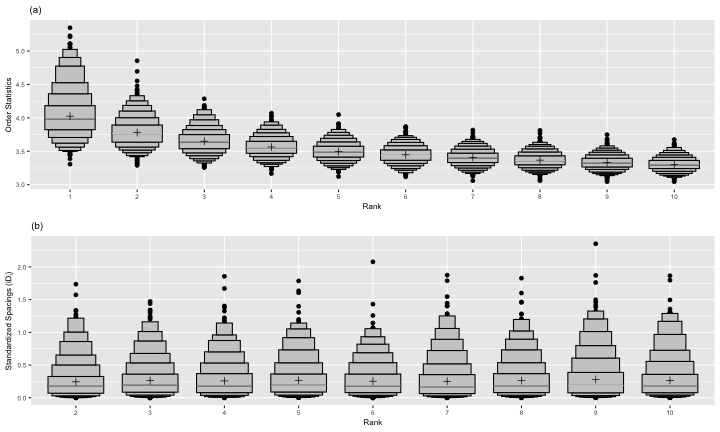
\includegraphics[width=1\linewidth]{figure/spacings-1} 

}

\caption{(a) Distribution of the descending order statistics $X_{i:n}$ and (b) distribution of the standardised spacings $iD_{i,n}$ for $i \in \{1,\dots,10\}$ for $1,000$ samples each containing $20,000$ random numbers from the standard normal distribution.}\label{fig:spacings}
\end{figure}

This theorem is illustrated using Figure \ref{fig:spacings}, which shows the distribution of the descending order statistics \((X_{i:n})\) and the standardized spacings, \((iD_{i,n})\), for \(i \in \left\{1,\dots,10\right\}\) for \(1,000\) samples each containing \(20,000\) random numbers from the standard normal distribution. Figure \ref{fig:spacings} (a) shows the distribution of \(X_{i:n}\) with means of \(X_{i:n}\) depicted as black crosses. The gaps between consecutive black crosses give the spacings between higher-order statistics \((D_{i,n})\). We note that the normal distribution is in the maximum domain of attraction of the Gumbel distribution and that this example contains no outliers. A consequence of Theorem \ref{thm:spacingtheorem} is that the standardised spacings \((iD_{i,n})\) for \((i = 1,\dots , K)\), are approximately iid \autocite{burridge2006additive}. Figure \ref{fig:spacings} (b) shows the distribution of the standardised spacings \((iD_{i,n})\) for \((i = 1,2,\dots,10)\) for \(1,000\) samples of size \(20,000\). Each letter-value box plot \autocite{hofmann2017value} exhibits approximately the shape of an exponential distribution.

\BeginKnitrBlock{definition}[Distribution of probability densities]
\protect\hypertarget{def:DPD}{}{\label{def:DPD} \iffalse (Distribution of probability densities) \fi{} }(Definition 6 in \textcite{hugueny2013novelty}, p.~105)

Let X be a (possibly multivariate) random variable with CDF \(F\), pdf \(f\), support \(D_{f}\), and probability space \(P_{f}\). \(Y=f(X)\) is a random variable, distributed according to:

\begin{center}
        $\forall y \in P_{f},\;\;G(y;f) = P(Y \leqslant y)$\\
    $\;\;\;\;\;\;\;\;\;\;\;\;\;\;\;\;\;\;\;\;\;\;\;\;\;\;\;\;\;\;\;\;\; = P(f(X) \leqslant y)$\\

            $\;\;\;\;\;\;\;\;\;\;\;\;\;\;\;\;\;\;\;\;\;\;\;\;\;\;\;\;\;\;\;\;\;\;\;\;\;\;\;\;\;\; =\int_{f^{-1}(]y_{min},y])}f(x)dx,$
\end{center}

where \(y_{min}=\text{Inf}(P_{f})\) and \(f^{-1}(]y_{min},y])\) is the preimage of
\(]y_{min},y]\) under \(f\).

\begin{flushright}
    $\square$
\end{flushright}
\EndKnitrBlock{definition}

\textbf{Proposition 1.1} (The domain of attraction of the distribution of probability density (DPD) for the multivariate Gaussian)

(Proposition 4 in \textcite{hugueny2013novelty}, p.~141; \emph{the notations have been changed for consistency within this thesis}.)

Let \(f\) be the multivariate Gaussian distribution. \(F\) is for the distribution of its minima in probability density in the domain of attraction of the minimum Weibull distribution \(\Psi_{\alpha}^{-}\).

For a sample size \(m\in N^{*}\), the norming constants can be chosen to be:

\begin{flushleft}
        $\;\;\;\;\;\;\;\;\;\;\;\;\;\;\;\;\;\;\;\;\;\;\;\;c_{m} = G^{\longleftarrow} (\frac{1}{m};f)$\\
        $\;\;\;\;\;\;\;\;\;\;\;\;\;\;\;\;\;\;\;\;\;\;\;\;d_{m} = 0$\\
    $\;\;\;\;\;\;\;\;\;\;\;\;\;\;\;\;\;\;\;\;\;\;\;\;\alpha_{m}=1$.
\end{flushleft}

\hypertarget{calculation-of-anomalous-threshold}{%
\subsection{Calculation of Anomalous Threshold}\label{calculation-of-anomalous-threshold}}

Chapter \ref{ch:stray} and Chapter \ref{ch:oddwater_features} both use Theorem \ref{thm:spacingtheorem} (Spacing Theorem by \textcite{weissman1978estimation}) to estimate a data-driven anomalous threshold to discriminate anomalies. This step sorts anomalous scores and searches for any large gap at the upper tail of the distribution defined by the anomalous scores. This search for significant gaps in the upper tail can either be performed using the top-down algorithm by \textcite{burridge2006additive} or bottom-up algorithm by \textcite{schwarz2008wind}.

\hypertarget{top-down-algorithm}{%
\subsubsection{Top-down algorithm}\label{top-down-algorithm}}

As the name implies, the top-down algorithm introduced by \textcite{burridge2006additive} starts from the maximum and moves backwards over the sorted array, seeking a significantly large gap. As summarised by \textcite{schwarz2008wind}, the top-down algorithm is as follows:

\begin{itemize}
\tightlist
\item
  Let \(X_{1},X_{2},\dots X_{n}\) be a sample from a distribution function \(F,\) and let \(X_{1:n}\geqslant X_{2:n}\geqslant \cdots \geqslant X_{n:n}\) be the order statistics.
\item
  Let \(D_{i} = X_{i:n} - X_{i+1:n}\) be the spacing between successive order statistics.
\item
  Calculate the standardised spacings, \(S_{i} \equiv iD_{i}\).
\item
  Find the maximum of the first \(N/\alpha\) spacings, \(S_{k}\), where \(N\) is the maximum possible number of outliers and \(\alpha\) is the acceptable false positive rate. The quantity \(N/\alpha\) then represents the number of spacings that must be examined to achieve a significance level of \(\alpha\).
\item
  If \(k \leq N\) spacings, mark the top \(k\) values as anomalies.
\item
  In addition to the gap between anomalous points and the valid data, sometimes there can be multiple gaps in between different groups of anomalous points. Therefore, repeat the above steps on the remaining data until no more gaps are found in the top \(N\) values.
\end{itemize}

However, repeating the process over data until it detects all the discrete groups of anomalies present in the dataset makes the algorithm inefficient for massive datasets with vast quantum of data. Further, it is not desirable to set a value for the maximum possible number of outliers, because this value is not known in advance for many real-world applications. Ideally, the algorithm should be able to pick all the anomalies present in the data without having this predetermined number. Further, according to \textcite{schwarz2008wind}, this algorithm does not use the full power of the spacing theorem; it only employs the fact that the standardised spacings are iid and fails to use the fact that they are exponentially distributed, which could have given more information about how unlikely is a given spacing. The bottom-up algorithm introduced by \textcite{schwarz2008wind} has the ability to release these unrealistic assumptions and overcome the limitations of the top-down algorithm. The bottom-up algorithm is based on the work of \textcite{burridge2006additive} but uses the full power of the spacing theorem.

\hypertarget{bottom-up-algorithm}{%
\subsubsection{Bottom-up algorithm}\label{bottom-up-algorithm}}

As in the top-down algorithm, the bottom-up algorithm is also based on the assumption that anomalies can bring large separations between valid data and anomalies, compared with the separations between valid data among themselves. However, in contrast to the top-down algorithm, the bottom-up algorithm now starts from the middle of the sorted data array, which represents the valid data, and moves forward towards the upper tail of the sorted array until it reaches a large gap, which is highly unlikely to occur if it is generated from the same distribution of the valid data. When a gap is encountered that is well beyond expectation, it terminates the searching process and marks all the points above that value as outliers. The specific steps of the bottom-up algorithm proposed by \textcite{schwarz2008wind} is as follows:

\begin{itemize}
\tightlist
\item
  Let \(X_{1},X_{2},\dots X_{n}\) be a sample from a distribution function \(F,\) and let \(X_{1:n}\geqslant X_{2:n}\geqslant \cdots \geqslant X_{n:n}\) be the order statistics.
\item
  Calculate \(D_{i} = X_{i:n} - X_{i+1:n}\), the spacing between successive order statistics.
\item
  At each rank \(i\), test the hypothesis that \(X_{i:n}\) is the largest valid data point in the sample, with the help of the spacings immediately below it (\(D_{i+1}, D_{i+2},..\)). If \(X_{i:n}\) is the largest valid data point in the sample, according to the spacing theorem, spacings \(D_{i}, D_{i+1}, D_{i+2},\dots\) should be proportional to \(1, \frac{1 }{2}, \frac{1 }{3},\dots\), and so on. This allows us to use spacings \(D_{i+1,n},D_{i+2,n}, \dots,D_{i+k,n}\) to predict the spacing \(D_{i}\):

  \begin{center}
            $\hat{D_{i}}=\frac{1}{k-1}\sum_{j=2}^{k}jD_{i+j-1}$
        \end{center}

  (Since the spacing theorem applies only to a small fraction of the data ranked near the upper tail, the entire dataset cannot be used to estimate \(D_{i}\) and therefore is used only \(k\)(\(\ll n\)) number of spacings for the estimation process. The value \(k\) should be large enough to obtain a stable estimate for \(D_{i}\), but small compared with the sample size, \(n\). \textcite{schwarz2008wind} has recommended \(50\) spacings as a rough guideline for the value \(k\) and the same has been used by \textcite{wilkinsonvisualizing} for large samples). If they all represent valid points, then all the terms in the summation have the same mean, which is similar to the mean of \(D_{i}\). Therefore, \(\hat{D_{i}}\) serves as an estimator for \(D_{i}\).
\item
  As in the spacing theorem, since \(D_{i}\) follows an exponential distribution with mean proportional to \(i^{-1}\), for a given significance level \(\alpha\), a threshold \(t\) that will not be exceeded by valid data can be obtained using:

  \begin{center}
            $t=\hat{D_{i}}log(1/ \alpha)$
        \end{center}
\item
  Work upward towards the upper tail of the sorted data array. At the first \(i\) where spacing \(D_{i}\) exceeds threshold \(t\), terminate the searching process and flag \(X_{i:n}\) and all the points above in the sorted array as outliers.
\end{itemize}

The bottom-up algorithm has been used in the research presented in Chapter \ref{ch:stray} and Chapter \ref{ch:oddwater_features} because of its obvious advantages over the top-down algorithm.

\hypertarget{motivation-and-objectives}{%
\section{Motivation and Objectives}\label{motivation-and-objectives}}

\label{sec:motivation}

In light of the increasing demand for accurate and powerful automated methods for early detection of anomalies in the streaming data scenario and the lack of attention paid to this topic, the primary motivation of this thesis is to develop methods for early detection of anomalies in the streaming data context.

The \textbf{first} motivation of this thesis arises from the recently proposed HDoutliers method by \textcite{wilkinsonvisualizing}. The HDoutliers algorithm is a powerful algorithm with a strong theoretical foundation for anomaly detection in high-dimensional data. However, some limitations significantly hinder its performance level. The effect of these limitations is a tendency to increase the rate of false positives and/or rate of false negatives under certain conditions. Therefore, the first objective is to propose solutions to these limitations of the HDoutliers algorithm. Chapter \ref{ch:stray} addresses this objective. The proposed algorithm, the stray algorithm, is based on distance measures and the extreme value theory. Chapter \ref{ch:stray} also demonstrates how the stray algorithm can assist in detecting anomalies in other data structures, such as time series data and streaming temporal data. The improved algorithm is implemented in the open source R package \texttt{stray}\}.

The \textbf{second} motivation of this thesis originated from the limited research attempts on detecting anomalous series within a large collection of series in the streaming data scenario where data flow rapidly in a continuous manner. A few researchers \autocite{hyndman2015large,wilkinsonvisualizing} have developed methods to identify anomalous series within a large collection of series, mainly focusing on the batch scenario where it is assumed that the entire dataset is available prior to analysis. However, in contrast to the batch scenario, the streaming data scenario poses many different challenges owing to its complex nature evolving over time. In addition to the obvious difficulties caused by the large volume and velocity of streaming data, highly noisy signals can increase the related complexity. Nonstationarity (concept drift) is another major topic in the streaming data analysis that makes it difficult to distinguish new typical behaviour from anomalous events \autocite{faria2016novelty}. To address this issue, detectors should be able to learn and adapt according to the conditions present. Early detection of anomalies as soon as they start but before they end is another major requirement of most applications related to this problem. Therefore, the second objective of this study is to develop a powerful automated method to detect anomalous series within a large collection of series in the streaming data context such that it meets these requirements. Chapter \ref{ch:oddstream} is dedicated to achieving this objective. This chapter presents a new algorithm based on density modelling and the extreme value theory. To cope with nonstationarity (concept drift), a density-based comparison approach is proposed. The proposed algorithm can detect significant changes in the typical behaviour and automatically update the anomalous threshold upon detecting a nonstationarity. The proposed algorithm is implemented in the open source R package \texttt{oddstream}.

The \textbf{third} motivation of this thesis arises owing to the non-existence of a customised method to detect technical anomalies in high-frequency water-quality data from \emph{in situ} sensors. Automated \emph{in situ} sensors have the potential to revolutionise the way we manage and monitor environmental settings, such as air, soil and water. The data produced by these sensors enable us to identify fine-scale patterns, trends and extremes over space and time. Although they represent cutting-edge technology, the data they produce are still prone to errors because of many reasons, such as miscalibration, biofouling and battery failures \autocite{horsburgh2015open}. Moreover, these anomalies and the ability to detect them can differ according to the geographic characteristics of the environmental system and the spatial placement of the sensors. To ensure data quality, we need to automate the real-time detection of anomalies. Therefore, our third objective is to propose a new framework for automated anomaly detection in high-frequency water-quality data from \emph{in situ} sensors.
Chapters \ref{ch:oddwater_features} and \ref{ch:oddwater_main} address this objective. In these chapters, an attempt was made to develop methods that can incorporate the correlation structure of several measurements taken from each site. This involves an application performing anomaly detection using turbidity, conductivity and river level data collected from rivers flowing into the Great Barrier Reef lagoon, Australia. The proposed algorithm is implemented in the open source R package \texttt{oddwater}.

Conclusions are drawn in Chapter \ref{ch:conclusion} with a discussion on potential extensions to the proposed algorithms introduced in Chapter \ref{ch:stray}, \ref{ch:oddstream} and \ref{ch:oddwater_features}.

These three main objectives guided the structuring and development of the major chapters of this thesis. Since this is a thesis by publication that has an introductory chapter and a concluding chapter with articles in between, the reader may notice some amount of repetition among chapters. Each article should be self-contained and therefore has been published with relevant materials for completeness.

\hypertarget{ch:stray}{%
\chapter{Anomaly Detection for High Dimensional Data}\label{ch:stray}}

\textbf{This article has been submitted to \emph{Computational Statistics \& Data Analysis} for possible publication.}

\includepdf[pages={1-30}, scale=1]{stray_paper_EBS.pdf}

\hypertarget{ch:oddstream}{%
\chapter{Anomaly Detection in Streaming Non-stationary Temporal Data}\label{ch:oddstream}}

\textbf{This article has been accepted for publication in the \emph{Journal of Computational and Graphical Statistics} and is currently in press}

Full paper is available at - \url{https://www.tandfonline.com/doi/abs/10.1080/10618600.2019.1617160?journalCode=ucgs20}

\hypertarget{ch:oddwater_features}{%
\chapter{\texorpdfstring{A Feature-Based Procedure for Detecting Technical Outliers in Water-Quality Data from \emph{in situ} Sensors}{A Feature-Based Procedure for Detecting Technical Outliers in Water-Quality Data from in situ Sensors}}\label{ch:oddwater_features}}

\textbf{This article has been revised and resubmitted to the "Water Resources Research* for possible publication. The work is based on the collaborative research project carried out with the Queensland University of Technology and the Queensland Department of Environment and Science, Great Barrier Reef Catchment Loads Monitoring Program from April to July 2018.}

\includepdf[pages={1-31}, scale=1]{oddwater.pdf}

\hypertarget{ch:oddwater_main}{%
\chapter{\texorpdfstring{A Framework for Automated Anomaly Detection in High Frequency Water-Quality Data From \emph{in situ} Sensors}{A Framework for Automated Anomaly Detection in High Frequency Water-Quality Data From in situ Sensors}}\label{ch:oddwater_main}}

\textbf{This article is published in the \emph{Science of the Total Environment}. The work is based on the collaborative research project carried out with the Queensland University of Technology and the Queensland Department of Environment and Science, Great Barrier Reef Catchment Loads Monitoring Program from April to July 2018. }

Full paper is available at - \url{https://www.sciencedirect.com/science/article/pii/S0048969719305662}

\hypertarget{ch:conclusion}{%
\chapter{Conclusion}\label{ch:conclusion}}

This thesis by publication is built around four articles. Although the four articles have their own focus motivated by a wide range of different analytical challenges from different fields, none of them is completely an anomaly. The four articles move around a unifying theme on anomaly detection in streaming time series data, with a different degree of attention to the common theme.

\hypertarget{summary-of-the-results-and-contributions}{%
\section{Summary of the Results and Contributions}\label{summary-of-the-results-and-contributions}}

Despite the long history of research on anomaly detection, the problem is still challenging owing to the evolving nature of the problem setting introduced by different applications and user requirements. This thesis is an attempt to reduce this gap by introducing three new algorithms, stray, oddstream and oddwater, for anomaly detection in temporal data with applications in pedestrian monitoring, security monitoring and sensor quality monitoring, respectively. The three algorithms stem from the analytical challenges introduced by the applications with various input data structures, definitions, problem specifications, user requirements, limitations of the state-of-the-art methods and unavailability of techniques that accommodate some of the data challenges.

\hypertarget{the-stray-algorithm}{%
\subsection{The stray algorithm}\label{the-stray-algorithm}}

Anomaly detection in high-dimensional data is a challenging yet important task, because it has applications in many fields. The HDoutliers algorithm by \textcite{wilkinsonvisualizing} is a powerful algorithm for anomaly detection in high-dimensional data with a strong theoretical foundation. However, it suffers from a few limitations since it limits the anomalous score calculation only to the nearest neighbour distances and uses the Leader algorithm to form several clusters of points prior to anomalous score calculation. The effect of these limitations is a tendency to reduce computational efficiency and increase false detection rates under certain circumstances. Therefore, the main objective of Chapter \ref{ch:stray} was to propose solutions to the limitation of the HDoutliers algorithm and thereby improve its capabilities.

The proposed algorithm, stray, addresses the limitations of the HDoutliers algorithm. In the stray algorithm, an anomaly is defined as an observation that deviates markedly from the majority with a large distance gap. It calculates an anomalous score for each data instance using \(k\)-nearest neighbour distances with the maximum gap. An approach based on extreme value theory is then applied to the anomalous scores to calculate a data-driven anomalous threshold. This improved algorithm can assign both a label and an anomalous score that explains the level of outlierness of each data instance.

This study offers two fundamental contributions. First, it proposes an improved algorithm for anomaly detection in high-dimensional data that addresses the limitations of the state-of-art-method, the HDoutliers algorithm. It outperforms the state-of-the-art method in both accuracy and computational efficiency. Among many other advantages, the stray algorithm has the ability to deal with the masking problem, multimodal distributions and inliers and outliers. The stray algorithm is specially designed for high-dimensional data. As the second contribution, the study demonstrates how the stray algorithm can assist in detecting anomalies present in other data structures, such as temporal data and streaming data, using feature engineering.

Since the stray algorithm is based on the distance definition of an anomaly, the algorithm expects data instances to have a clear distance separation between the anomalous and typical points. Then, only the anomalous points (if any) have significantly large k-nearest neighbour distances with the maximum gap that discriminate anomalies from typical points. However, some applications do not exhibit large gaps between typical points and anomalies. Instead, the anomalies deviate from the majority, or the region of typical data, gradually, without introducing a large distance between typical and anomalous points. In the absence of clear distance separation between anomalous points and the typical points, the stray algorithm fails to detect anomalies since distance measures are the primary source of information for the algorithm to detect anomalies. This limitation of the stray algorithm motivates the second algorithm proposed in Chapter \ref{ch:oddstream} of this thesis.

\hypertarget{the-oddstream-algorithm}{%
\subsection{The oddstream algorithm}\label{the-oddstream-algorithm}}

In addition to the aforementioned limitation of the stray algorithm, the limited research attempts for detecting anomalous series within a large collection of streaming data motivated the second algorithm of this thesis, the oddstream algorithm. The primary focus of Chapter \ref{ch:oddstream} was to develop a powerful automated method to detect anomalous series within a large collection of series in the streaming data context.

In the oddstream algorithm, an anomaly is defined as an observation that is very unlikely, given the recent distribution of a given system. In this algorithm, a boundary for the system's typical behaviour is defined using extreme value theory. Then, a sliding window is used to test newly arrived data. The model uses time series features as inputs and a density-based comparison to locate nonstationarity. This algorithm can detect significant changes in the typical behaviour and automatically update the anomalous threshold on detecting nonstationarity.

This study offers three fundamental contributions. First, it proposes a new framework that provides early detection of anomalies within a large collection of streaming time series data. Second, it proposes a novel approach that adapts to nonstationarity. Third, using various synthetic and real datasets, it demonstrates the wide applicability and usefulness of the algorithm. Application of the oddstream algorithm with data obtained using fibre optic cables for intrusion detection showed that the algorithm has the ability to deal with large nonstationary streaming data that may have multimodal distributions.

\hypertarget{the-oddwater-algorithm}{%
\subsection{The oddwater algorithm}\label{the-oddwater-algorithm}}

Automated \emph{in situ} sensors have the potential to revolutionise the way we monitor environmental conditions. However, the data produced by these sensors are prone to errors because of many reasons, such as miscalibration, biofouling and battery failures \autocite{horsburgh2015open}. These technical outliers make the data unreliable for scientific analysis. Therefore, to ensure water-quality sensors yield high-quality data, we need to automate the real-time detection of technical outliers in such data. However, a customised method to detect technical outliers in water-quality data from \emph{in situ} sensors is lacking. No exiting outlier detection method is able to address this challenge owing to the complex nature of the definition of a technical outlier in water-quality data from \emph{in situ} sensors. Therefore, the main objective of Chapters \ref{ch:oddwater_features} and
\ref{ch:oddwater_main} was to propose a new framework to detect technical outliers in high-frequency water-quality data from \emph{in situ} sensors.

This study proposes an automated framework that provides early detection of technical outliers, caused by technical issues, in water-quality data from \emph{in situ} sensors. We compare two approaches to this problem: (1) using forecasting models (Chapter \ref{ch:oddwater_main}) and (2) using feature vectors with extreme value theory (Chapter \ref{ch:oddwater_features}). In the forecasting models, observations are identified as outliers when they fall outside the bounds of an established prediction interval. Two strategies are considered for this comparison study: anomaly detection (AD) and anomaly detection and mitigation (ADAM) for the detection process. With ADAM, the detected outliers are replaced with the forecast prior to the next prediction, whereas AD simply uses the previous measurements without altering detected outliers. The feature-based framework first identifies the data features that differentiate outlying instances from typical behaviours. Then, statistical transformations are applied to make the outlying instances stand out in transformed data space. Unsupervised outlier scoring techniques are then applied to the transformed data space. An approach based on extreme value theory is used to calculate a threshold for each potential outlier. The proposed frameworks are evaluated using two datasets obtained from \emph{in situ} sensors in rivers flowing into the Great Barrier Reef lagoon.

The feature-based approach (in Chapter \ref{ch:oddwater_features}) successfully identified outliers involving abrupt changes in turbidity, conductivity and river level, including sudden spikes, sudden isolated drops and level shifts, while maintaining very low false detection rates. Since this is an unsupervised algorithm, it can be easily extended to other water-quality variables, other sites and also to other outlier detection tasks in other application domains. The only requirement is to select suitable transformation methods according to the data features that differentiate the outlying instances from the typical behaviours of a given system. The transformations used in this study were mainly chosen as appropriate to the data collected from Sandy Creek and Pioneer River. Domain-specific knowledge plays a vital role when selecting suitable transformations.

\hypertarget{future-work}{%
\section{Future Work}\label{future-work}}

Since this is a thesis by publication, each article should be self-contained and therefore has been published with all the relevant possible further research directions discussed in detail. To avoid repetition, this section summarises only the key future research priorities, which are deemed underrepresented in the current literature.

While the HDoutliers algorithm is powerful, several classes of counterexamples were identified where the structural properties of the data did not enable the HDoutliers algorithm to detect certain types of outliers. However, I acknowledge that these counterexamples are not diverse and challenging enough to generalise the findings to conclude that stray is always the superior algorithm. Therefore, an important open research problem is to assess the effectiveness of these algorithms across the broadest possible problem space defined by different datasets with diverse properties \autocite{kang2017visualising}. It would also be interesting to explore how other classes of problems with various structural properties can influence the performance of the stray algorithm and where its weaknesses might lie. This type of instance space analysis \autocite{smith2014towards} will enable further insights into improved algorithm design.

In the oddstream algorithm, the use of the feature-based representation of time series is recommended, owing to its many advantages over the instance-based representation of time series. In the present study, only 14 features were used to represent a given time series. Further exploration of feature extraction and automatic feature selection methods is required to create a richer feature space that is suitable for many applications in the streaming data context. The proposed algorithm uses the first two principal components to obtain a two-dimensional feature space, and then defines an anomalous threshold on the resulting two-dimensional feature space. It is expected that in further studies, other dimension reduction techniques will be used, such as multidimensional scaling and random projection, to investigate the effects of such techniques on the performance of the proposed framework. Further, the density estimation in the proposed algorithm was performed using a bivariate kernel density estimation
method. Since the density values in the tail are used to build the model of the typical behaviour, additional experiments need to be conducted on density estimation methods, to improve the tail estimation. On this topic, the log-spline bivariate density estimation method and the local likelihood density estimation method will be considered, with the aim of achieving a better tail estimation, and thereby improving the performance of the proposed algorithm.
The current algorithm is developed under the assumption that the measurements produced by sensors are one-dimensional. Rapid advances in hardware technology have made it possible for many sensors to capture multiple measurements simultaneously, leading ultimately to a collection of multidimensional multivariate streaming time series data. Therefore, an important open research problem is to extend the oddstream algorithm to handle multidimensional, multivariate streaming data. Extending the oddstream algorithm to the detection of anomalies in this data context may allow us to perform anomaly detection in an even wider range of application domains.

Spatiotemporal anomaly detection for water-quality data also lags behind that for other \emph{in situ} sensor data types \autocite[e.g., air quality or meteorology;][]{wu2008spatio} because river data pose new challenges, such as the complex relationships between neighbouring sensors due to branching networks and flow directionality, tendency for biofouling and the highly dynamic nature of river water even under typical conditions \autocite{kang2009discovering}. These challenges make traditional anomaly detection approaches inadequate for spatiotemporal water-quality data and require new methods. The oddwater algorithm is expected to expand into space and time so that it can deal with the spatiotemporal correlation structure along branching river networks. This will in turn provide a fundamental step-change in scientific understanding of the spatiotemporal dynamics of water quality in rivers and their networks and the potential downstream effects of pollutant loads.

\hypertarget{research-reproducibility}{%
\section{Research Reproducibility}\label{research-reproducibility}}

Research reproducibility is an important topic in modern science because it provides a general schema and an infrastructure to regenerate quantitative scientific results using the original datasets and methods \autocite{stodden2014implementing}. Therefore, to facilitate reproducibility and reuse of the results presented in this thesis, I undertook several actions under the three key areas: software, data and papers \autocite{stodden2014implementing}.

\hypertarget{software}{%
\subsection{Software}\label{software}}

This thesis introduces three R packages for anomaly detection.

The first R package is an accompaniment to the algorithm proposed in Chapter \ref{ch:stray} and includes useful functions for detecting anomalies in high-dimensional data. Version 1.0.0.9000 of the package was used for the results presented in Chapter \ref{ch:stray} and is available from GitHub at \url{https://github.com/pridiltal/stray}.

The second R package, \pkg{oddstream}, is an accompaniment to the algorithm proposed in Chapter \ref{ch:oddstream} and includes useful functions for detecting anomalous series within a large collection of streaming time series data. Version 0.5.0 of the package was used for the results presented in Chapter \ref{ch:oddstream} and is available from GitHub at \url{https://github.com/pridiltal/oddstream}.

The third package is an accompaniment to the algorithm proposed in Chapters \ref{ch:oddwater_features} and \ref{ch:oddwater_main} and includes useful functions for detecting technical anomalies in water-quality data from \emph{in situ} sensors. Version 0.5.0.9000 of the package was used for the results presented in Chapters \ref{ch:oddwater_features} and \ref{ch:oddwater_main} and is available from GitHub at \url{https://github.com/pridiltal/oddwater}.

\hypertarget{data}{%
\subsection{Data}\label{data}}

All the datasets on which the results are computed in each article are available via the corresponding R package. A Shiny web application available through the \texttt{oddwater} R package provides greater visual insight into the water-quality data from \emph{in situ} sensors and was heavily used during the labelling process to pinpoint observations.

\hypertarget{papers}{%
\subsection{Papers}\label{papers}}

The three main articles in Chapters \ref{ch:stray}, \ref{ch:oddstream} and \ref{ch:oddwater_features} describe the corresponding algorithms in detail and compare their implementations using various datasets. The source files, including datasets and R code to reproduce all figures, tables and analysis of each article, can be found in the following public GitHub repositories.

Chapter \ref{ch:stray}: `Anomaly Detection for High Dimensional Data' at \url{https://github.com/pridiltal/stray_manuscript}.

Chapter \ref{ch:oddstream}: `Anomaly Detection in Streaming Non-stationary Temporal Data' at \url{https://github.com/pridiltal/oddstream_manuscript}.

Chapters \ref{ch:oddwater_features}: `A Feature-Based Procedure for Detecting Technical Outliers in Water-Quality Data from \emph{in situ} Sensors' at \url{https://github.com/pridiltal/oddwater_manuscript}.

These articles were written entirely using \texttt{Rmarkdown} \autocite{Rmarkdown1}, and compiled into a thesis using the \texttt{bookdown} R package \autocite{Rbookdown1}, with the Monash PhD thesis rmarkdown template available at \url{https://github.com/robjhyndman/MonashThesis}. The source files of this thesis are available at \url{https://github.com/pridiltal/PhD_Thesis_2019}.

\printbibliography[heading=bibintoc]



\end{document}
